\newpage
\pagenumbering{roman} 
\setcounter{page}{1}
\appendix
\renewcommand\thechapter{A}

\chapter{Eddy Current Brake Calculations}

\begin{figure}[H]
	\begin{center}
		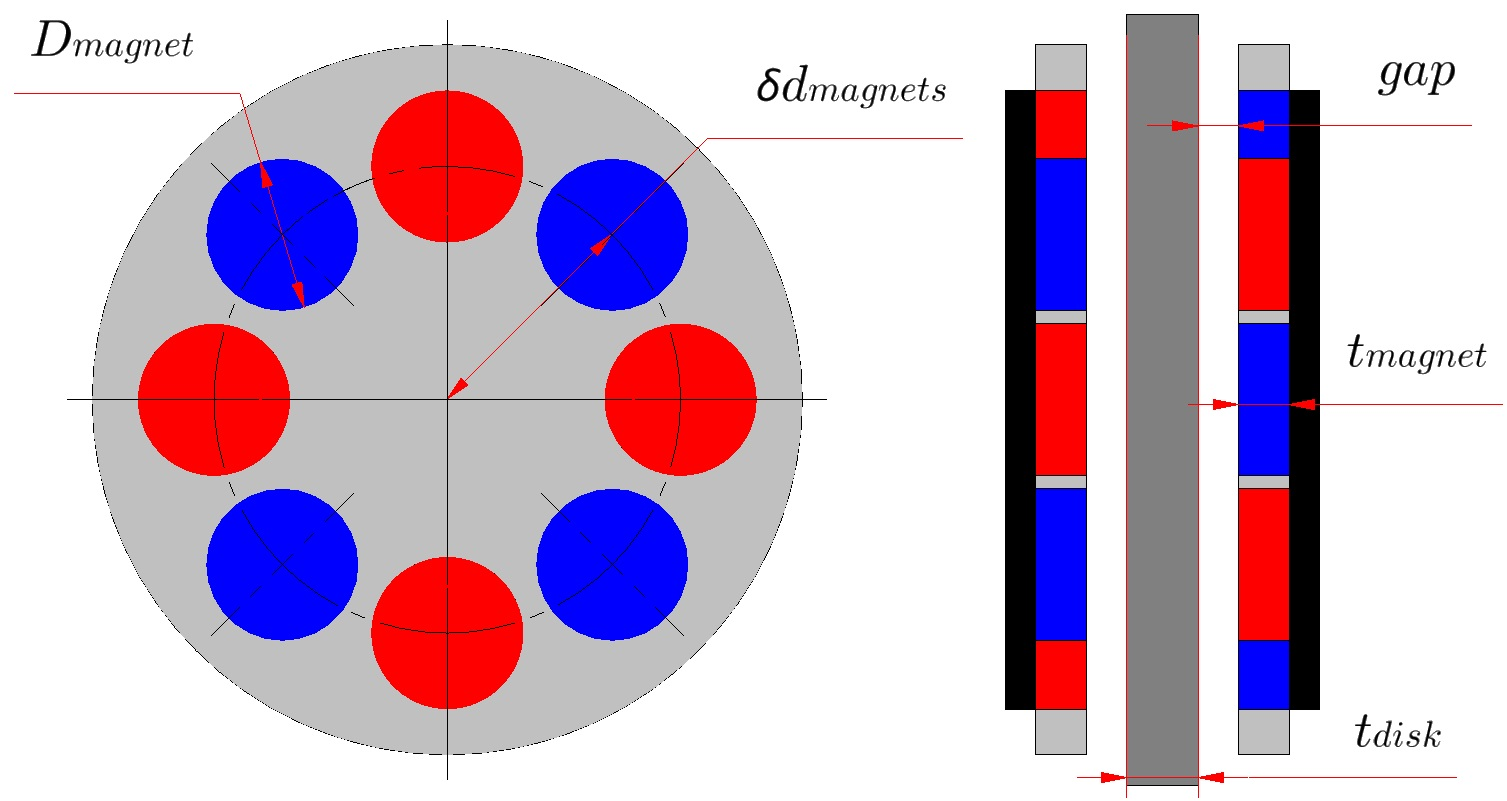
\includegraphics[width=0.8\textwidth]{Brake Layout.jpg}
		\caption{Eddy Current Brake Dimensions}
		\label{fig:EB}
	\end{center}
\end{figure}

\newpage

%At low speeds:\\
%The Eddy Currents in the Aluminium disc will be:
%\[
%\acs{I}_e = \frac{\acs{condDisk} \acs{B} \acs{v}}{2}
%\]
%The eddy currents within the disc is then:
%\[
%di = \frac{\acs{I}_e}{2 \pi} d\acs{theta}
%\]
%Using Ampere's Law, the force on an element at length l is then:
%\[
%d\acs{F} = \acs{B} \, di \, dl
%\]
%\[
%d\acs{T} = l \, d\acs{F}
%\]
%Thus, combining all these, we get:
%\[
%d\acs{T} = \frac{\acs{B} \, \acs{I}_e}{2 \pi} \, l \, d\acs{theta} \, dl
%\]
%By integrating, we get:
%\[
%\int_{0}^{R} \int_{0}^{2 \pi} \frac{\acs{B} \, \acs{I}_e}{2 \pi} \, l \, d\acs{theta} \, dl
%\]
%\[
%\acs{T} = \frac{\acs{condDisk}\acs{B}^2\acs{omega}_n R^2}{6}
%\]

\begin{figure}[H]
	\begin{center}
		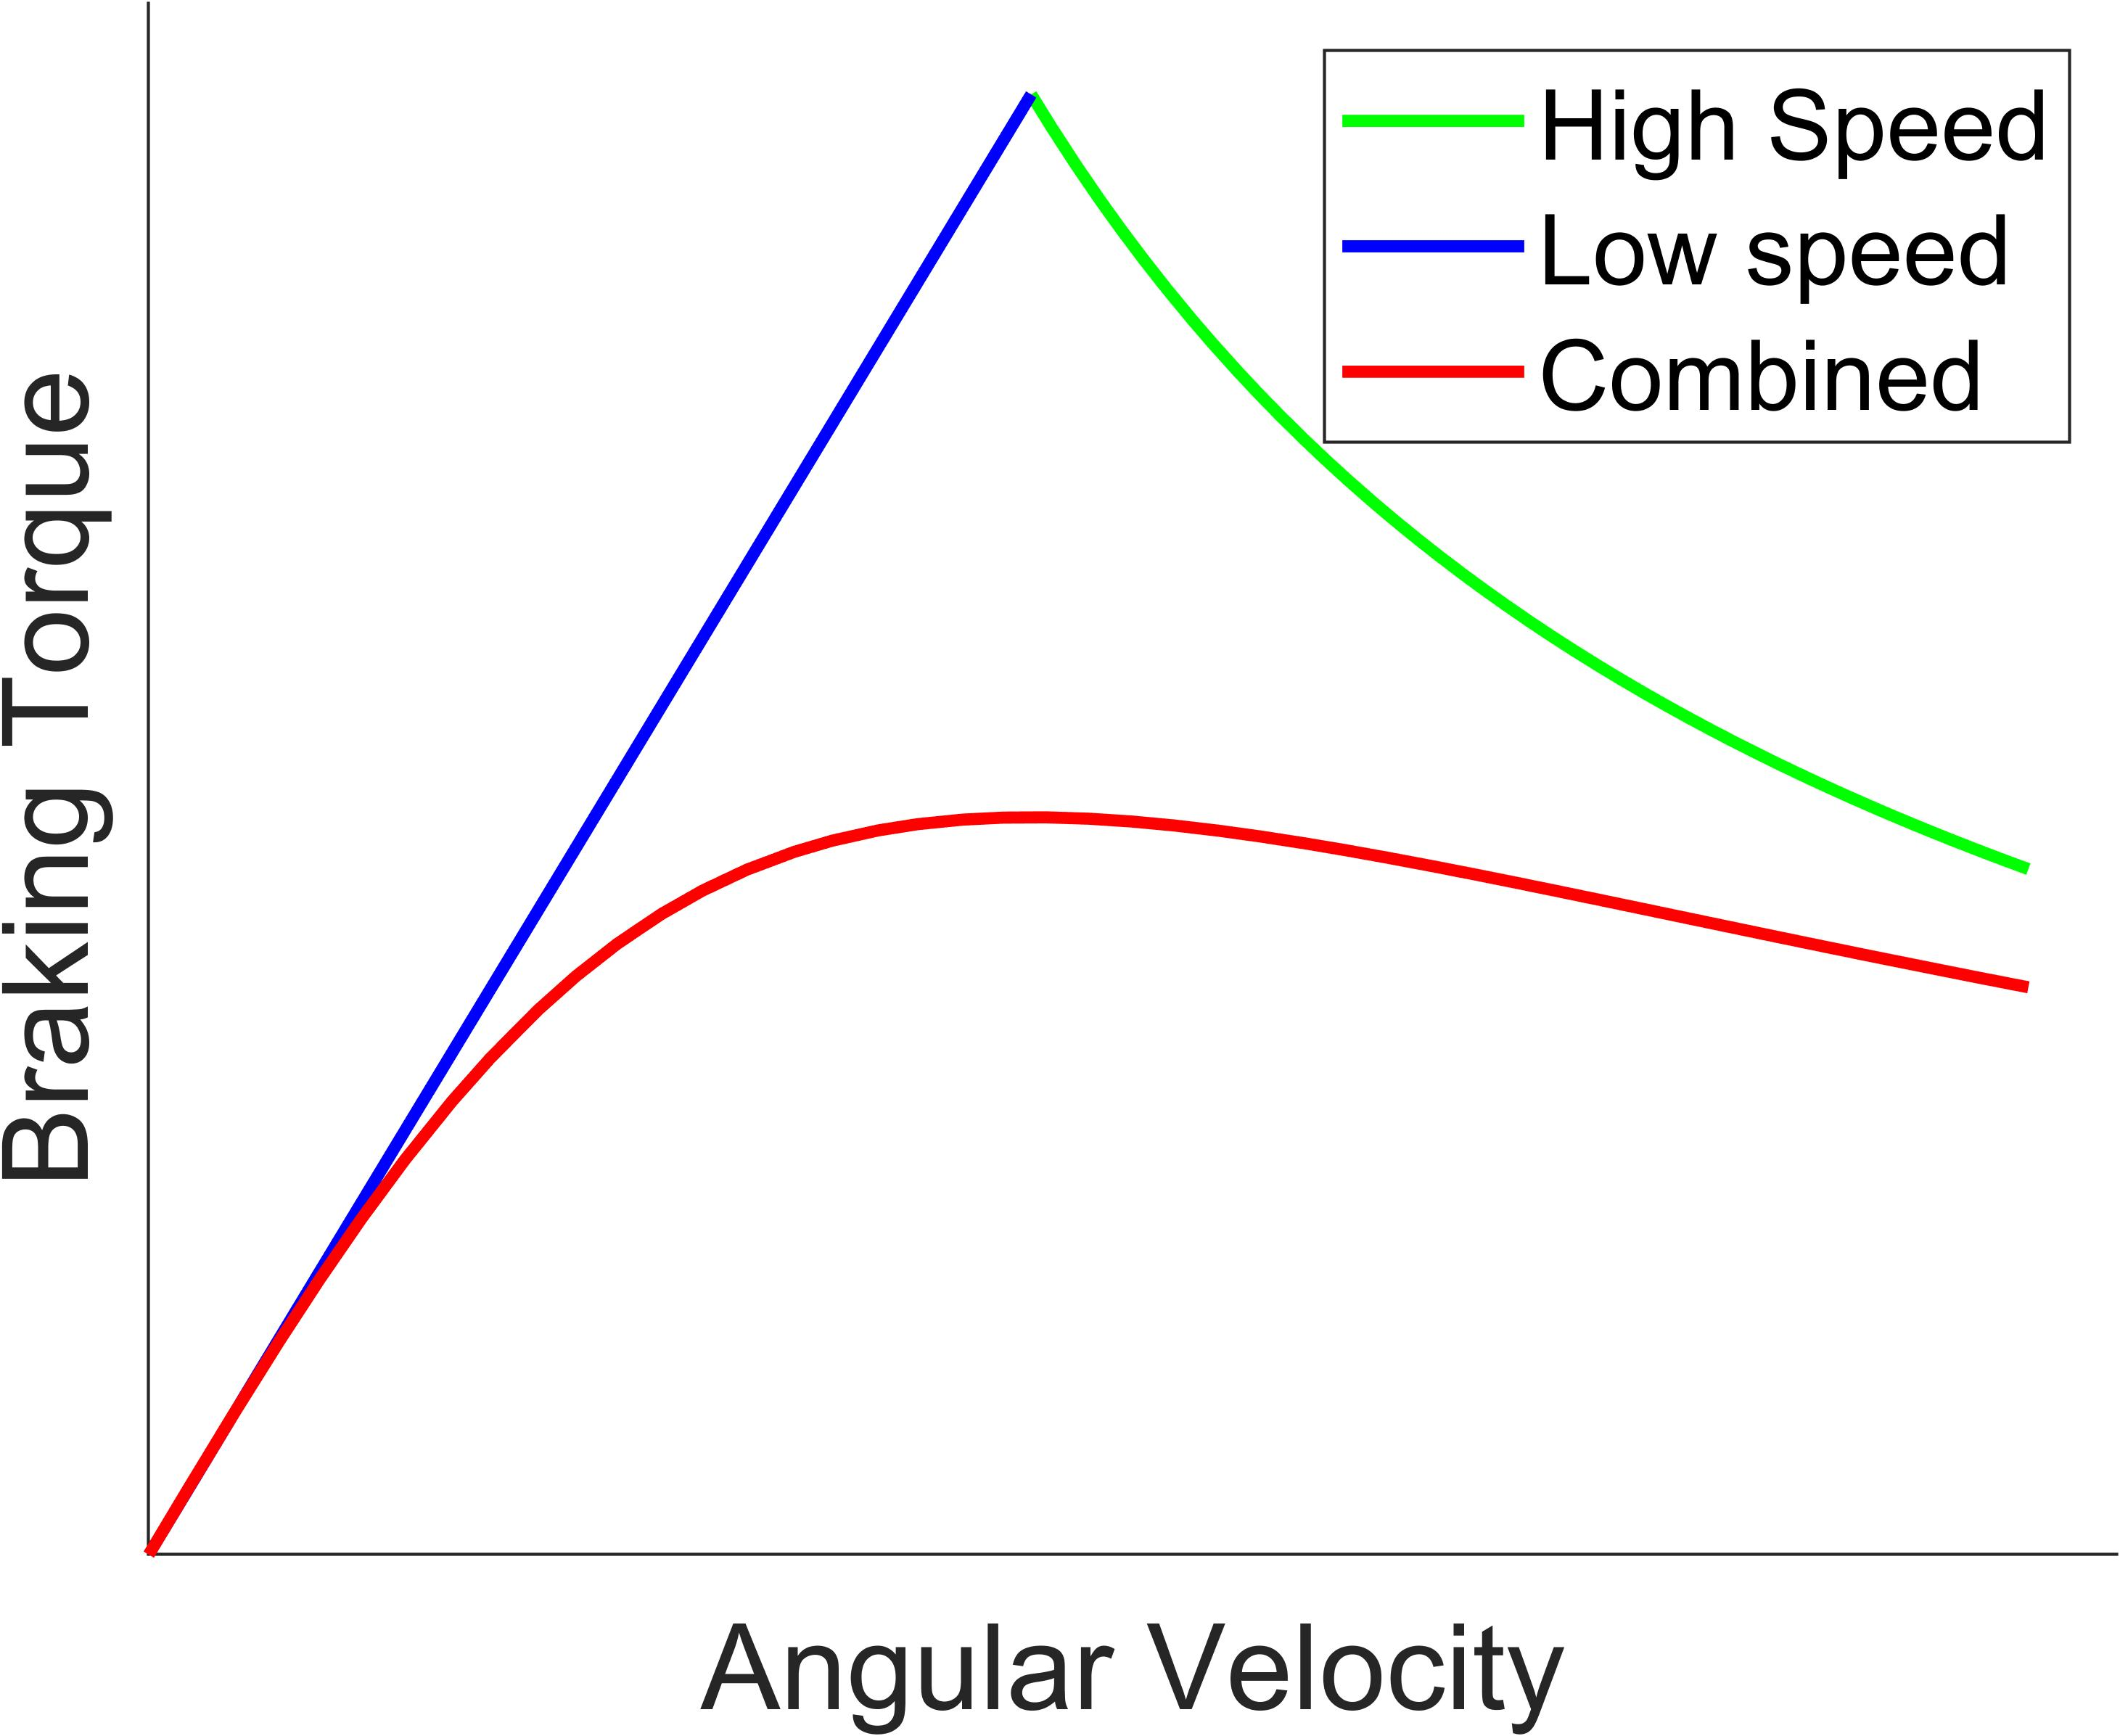
\includegraphics[width=0.8\textwidth]{Fig5.jpg}
		\caption{Figure 5}
		\label{fig:5}
	\end{center}
\end{figure}

\begin{figure}[H]
	\begin{center}
		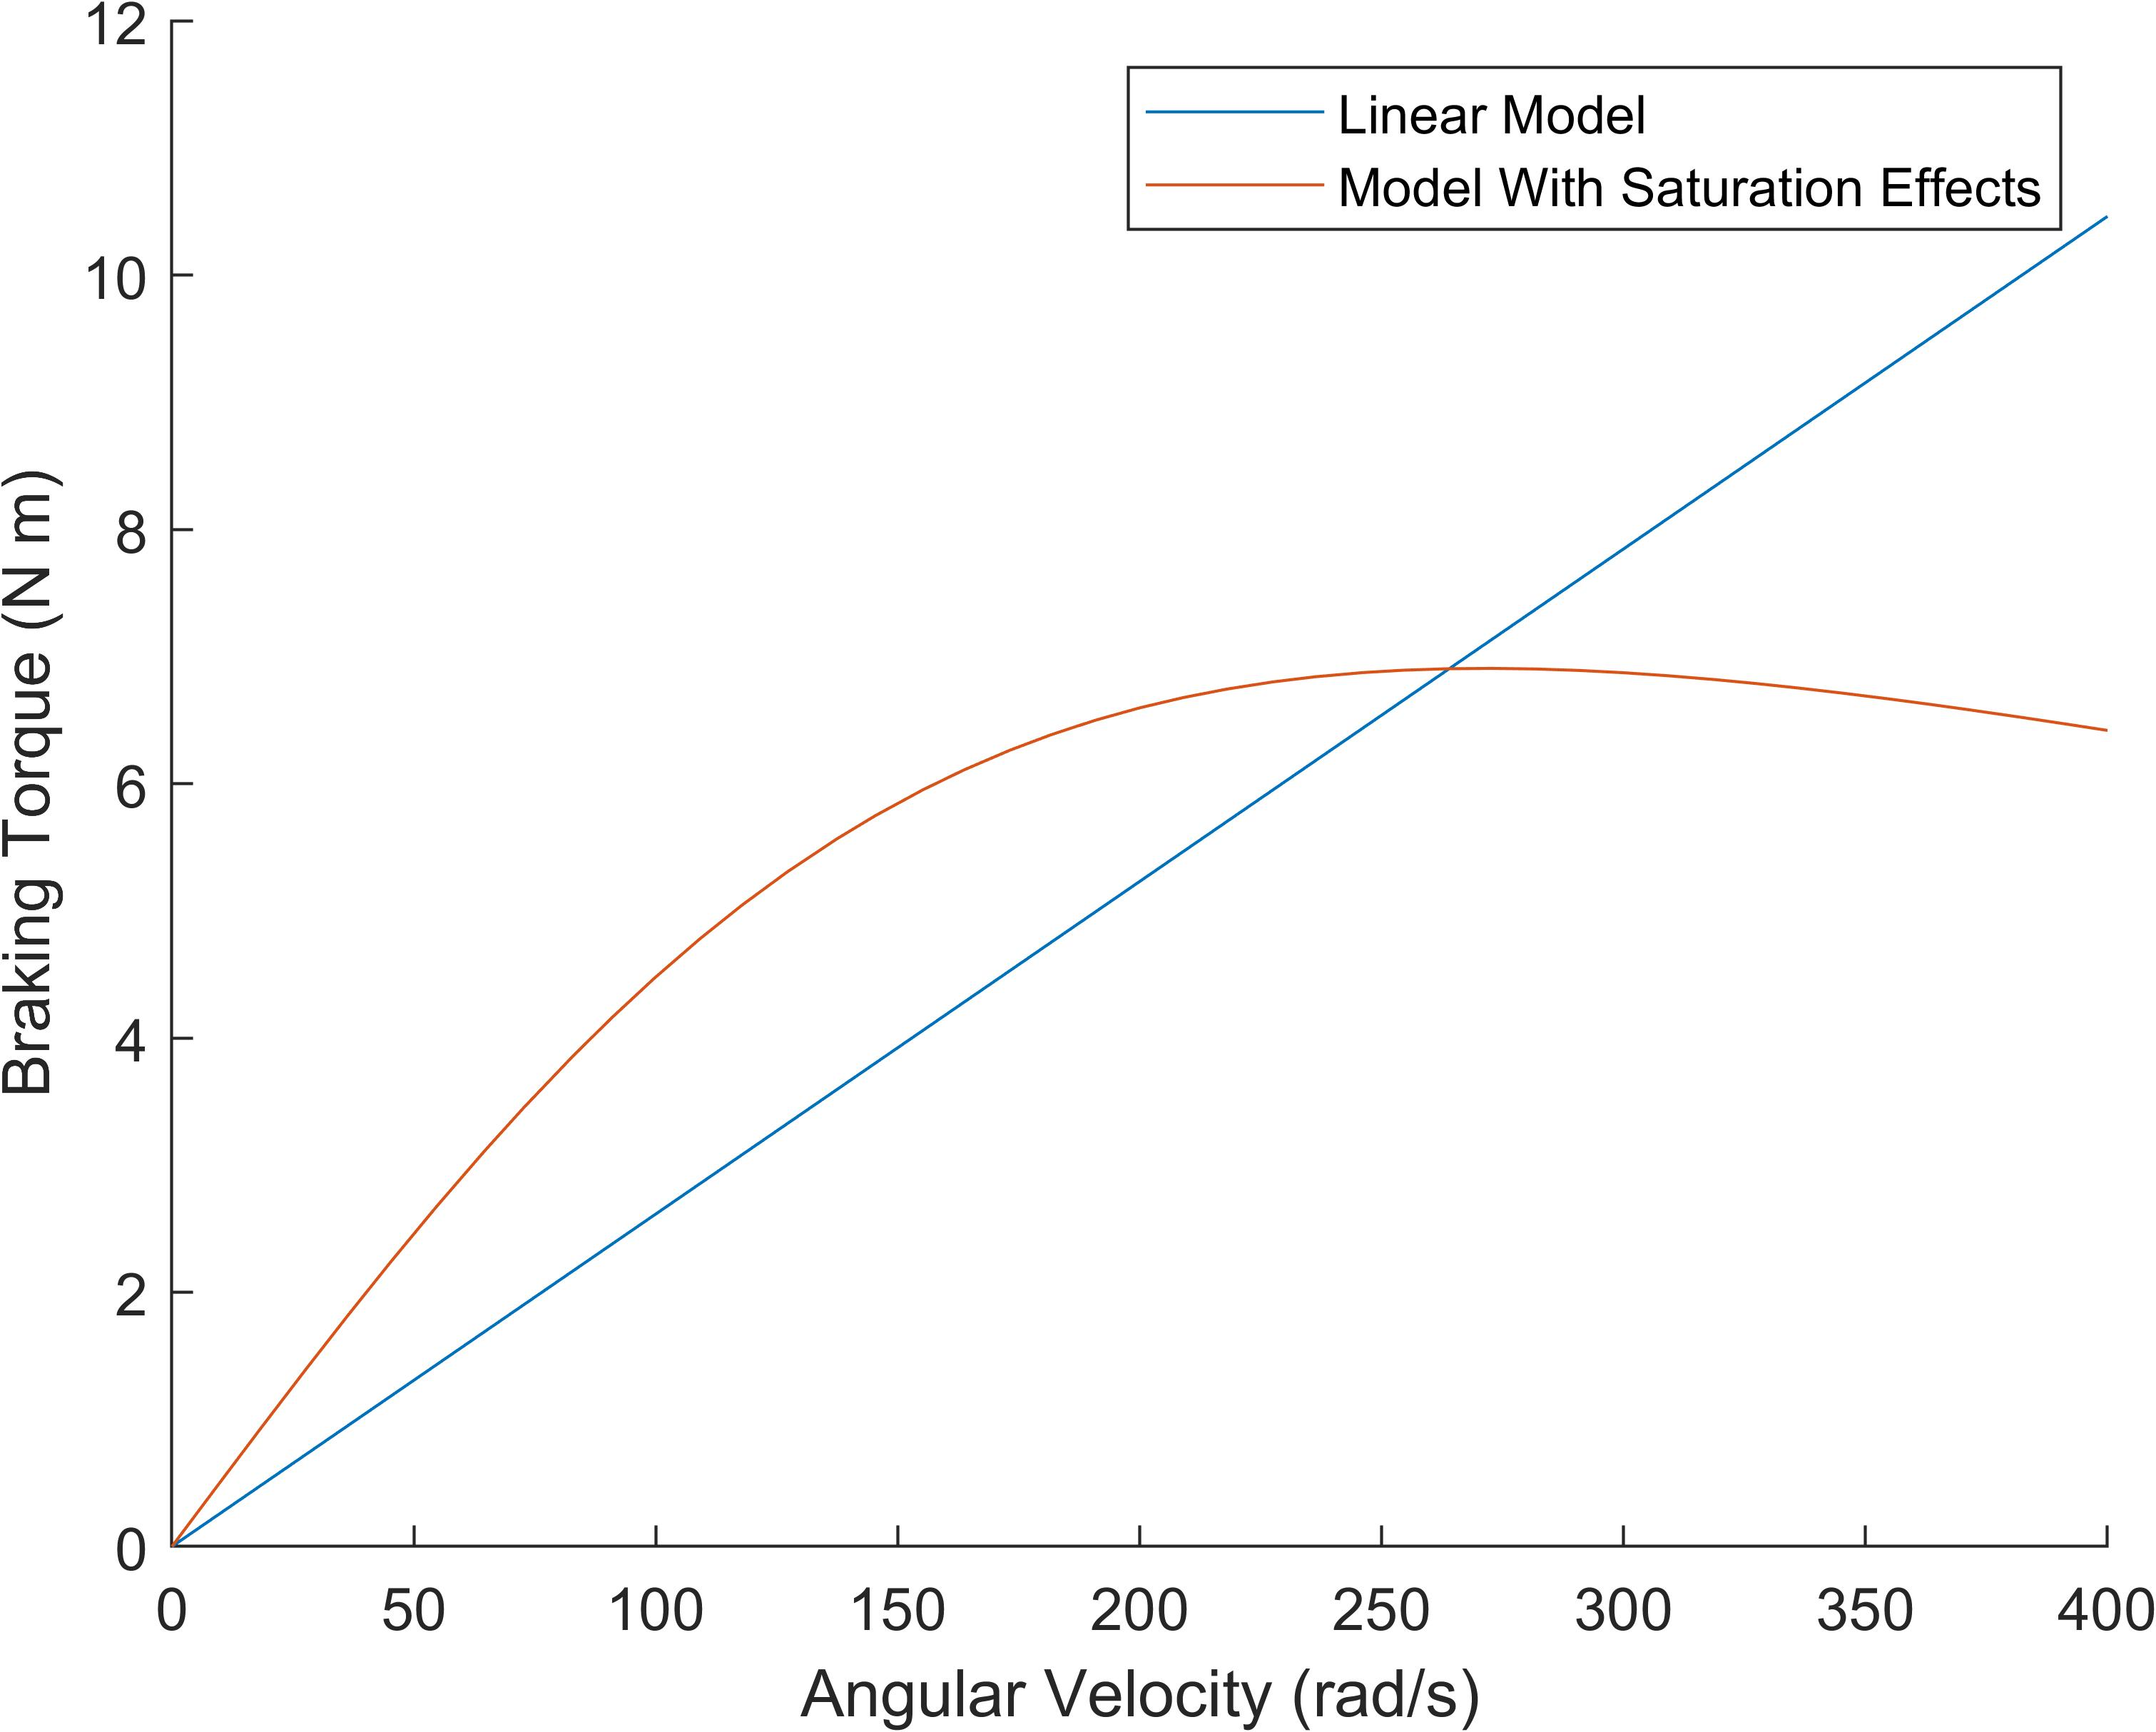
\includegraphics[width=0.8\textwidth]{Fig6.jpg}
		\caption{Figure 6}
		\label{fig:6}
	\end{center}
\end{figure}